\section{Auswertung}
\label{sec:Auswertung}

Im Folgenden findet die Auswertung der aufgenommenen Daten statt.
Dabei wird zunächst auf die Kompensation des lokalen Magnetfelds eingegangen
und über die Berechnung der Landé-Faktoren der Kernspin der Isotope bestimmt.
Schließlich wird das Isotopenverhältnis ermittelt
und schließlich die Größe des quadratischen Zeeman-Effektes abgeschätzt. 

\subsection{Magnetfeld der Erde}
\label{sec:Magnetfeld}

Um die Einflüsse des lokalen Erdmagnetfelds zu kompensieren,
wird das angelegte horizontale Magnetfeld,
bestehend aus Sweep- und Horizontalanteil, ermittelt.
Dies geschieht bei dem vorliegendem Helmholtzspulenpaar 
mithilfe der Gleichung für die magnetische Flussdichte
\begin{equation} \label{eq:helmholtz}
    B=\mu_0 \frac{8 I N}{\sqrt{125} A} \, ,
\end{equation}
wobei $\mu_0$ die magnetische Feldkonstante, $N$ die Windungszahl der jeweiligen Spule und $A$ der Radius ist.

Der im Frequenzbereich gemessene Strom $I$ ergibt sich dabei aus der Messung der Spannung des Sweepanteils (Startfeld) $U_\text{S}$
und der des Horizontalanteils $U_\text{H}$.
Aus diesen Spannungen können mithife des Ohmschen Gesetzes $U = R \cdot I$ die Ströme der Anteile berechnet werden.
Die Sweep-Spule hat einen mittleren Radius von $A_\text{S} = \qty{0.1639}{m}$,
eine Windungszahl von $N_\text{S} = 11$
und einen Widerstand von  $R_\text{S} = \qty{1}{\ohm}$
während die Horizontalanteilspule $A_\text{H} = \qty{0.1579}{m}$, $N_\text{H} = 154$ und $R_\text{H} = \qty{0.5}{\ohm}$ hat.
Daraus lassen sich die jeweiligen Strömstärken und addierten magnetischen Flussdichten in \autoref{tab:strom} berechnen.
\begin{table}
    \centering
    \caption{Die umgerechneten Stromstärken der Anteile des RF-Feldes beider Isotope.}
    \label{tab:strom}
    \begin{tabular}{c c c c c c c}
        \toprule 
        & \multicolumn{3}{c}{$\ce{^{85}_{}Rb}$} &
        \multicolumn{3}{c}{$\ce{^{87}_{}Rb}$} \\
        \cmidrule(lr){2-4}\cmidrule(lr){5-7}
    
        $f \mathbin{/} \mathrm{kHz}$ &
        $I_\text{S} \mathbin{/} \unit{\milli\ampere}$ &
        $I_\text{H} \mathbin{/} \unit{\milli\ampere}$ &
        $B \mathbin{/} \unit{\micro\tesla}$ &
        $I_\text{S} \mathbin{/} \unit{\milli\ampere}$ & 
        $I_\text{H} \mathbin{/} \unit{\milli\ampere}$ &
        $B \mathbin{/} \unit{\micro\tesla}$ \\
        \midrule
        100,0 &   660,0 &      0,0 &      39,83 &   764,0 &      0,0 &      46,11 \\
        200,0 &   652,0 &     16,0 &      53,38 &   888,0 &     16,0 &      67,62 \\
        300,0 &   486,0 &     44,0 &      67,92 &   842,0 &     44,0 &      89,40 \\
        400,0 &   409,0 &     66,0 &      82,56 &   883,0 &     66,0 &     111,17 \\
        500,0 &   375,0 &     84,0 &      96,30 &   967,0 &     84,0 &     132,02 \\
        600,0 &   224,0 &    112,0 &     111,74 &   938,0 &    112,0 &     154,83 \\
        700,0 &   164,0 &    132,0 &     125,66 &   993,0 &    132,0 &     175,68 \\
        800,0 &   295,0 &    140,0 &     140,58 &   629,0 &    184,0 &     199,32 \\
        900,0 &   269,0 &    158,0 &     154,79 &   357,0 &    226,0 &     219,74 \\
       1000,0 &   590,0 &    158,0 &     174,17 &   586,0 &    236,0 &     242,33 \\
        \bottomrule
    \end{tabular}        
\end{table}

Um die Horizontalkompenente des lokalen Erdmagnetfelds zu bestimmen,
werden diese gemessenenen Feldstärken in linearer Form angähert. 
Die Auslgeichsgeraden sind in \autoref{fig:geraden} zu finden.
\begin{figure}
    \centering
    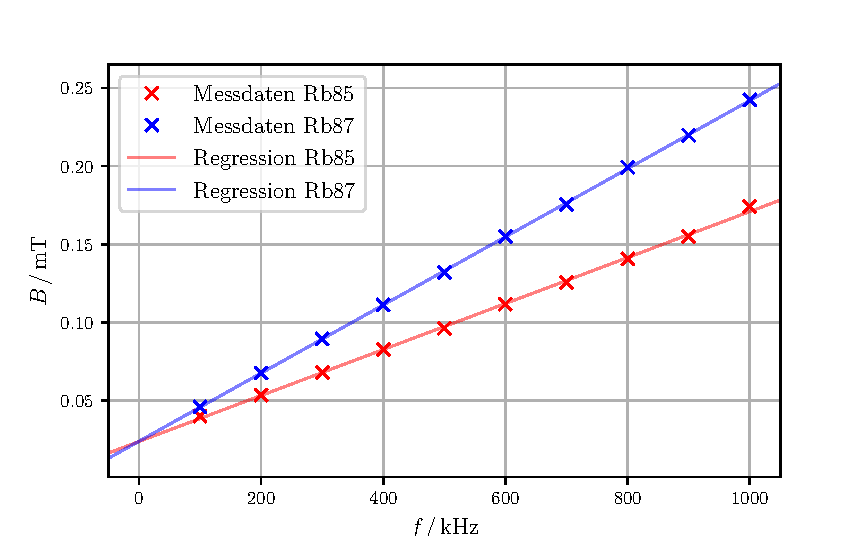
\includegraphics[width = 0.8\linewidth]{build/geraden.pdf}
    \caption{Die gemessenen Magnetfeldstärken sowie deren lineare Regression für beide Isotope.}
    \label{fig:geraden}
\end{figure}
Die Parameter ergeben sich dabei zu 
\begin{table}
    \centering
    \caption{Die Parameter der Auslgeichsrechnung für beide Isotope.}
    \begin{tabular}{c c c}
        \toprule 
        Isotop &
        $a \mathbin{/} \unit{\milli\tesla\per\kilo\hertz}$ &
        $b \mathbin{/} \unit{\milli\tesla}$ \\
        \midrule
        $\ce{^{85}_{}Rb}$ & $\num{0.000147(2)}$ & $\num{0.023792(1015)}$ \\
        $\ce{^{87}_{}Rb}$ & $\num{0.000218(1)}$ & $\num{0.023928(418)}$ \\
        \bottomrule
    \end{tabular}
\end{table}

Die Schnittpunkte beider Regressionsgeraden mit der Y-Achse ergeben
nach einer Mittelung das natürliche Magnetfeld der Erde zu
\begin{equation*}
    B_\text{H} = \qty{0.0239(5)}{\milli\tesla} \, .
\end{equation*}


\subsection{Landé-Faktoren}

Mithilfe der ermittelten Steigungen $a$ der beiden Auslgeichsgeraden können nun
die dazugehörigen Landé-Faktoren bestimmmt werden.
Dazu wird \autoref{eq:landefaktor} nach $g_\text{F}$ umgestellt:
\begin{equation*}
    \begin{aligned}
    \omega_0=\underbrace{g_F \frac{\mu_B}{h}}_{a^{-1}} B_0 & \Rightarrow a=\frac{h}{\mu_B g_F} \\
    & \Leftrightarrow g_F=\frac{h}{\mu_B a}
    \end{aligned}
\end{equation*}

Damit ergeben sich die Landé-Faktoren sowie deren Verhältnis zu
\begin{equation*}
    \begin{aligned}
        g_{\text{F}_{85}} &= \num{0.486(5)} \, , \\
        g_{\text{F}_{87}} &= \num{0.3278(10)} \quad \text{und} \\
        \frac{g_{\text{F}_{85}}}{g_{\text{F}_{87}}} &= \num{1.482(17)} \, .  
    \end{aligned}
\end{equation*}


\subsection{Kernspins}

Für die Berechnung der Kernspins wird zunächst mithife von \autoref{eq:g_J} der Landefaktor berechnet.
Für die Quantenzahlen $S=\frac{1}{2}$, $L=0$ und $J=L+S=\frac{1}{2}$ ergibt sich demnach $g_\text{J} = 2$ \cite{optical_pumping}.
Nach Umstellen von \autoref{eq:g_F} ergibt sich der Kernspin zu
\begin{equation}
    I=\frac{g_\text{J}}{4 g_\text{F}}-1+\sqrt{\left(\frac{g_\text{J}}{4 g_\text{F}}-1\right)^2+\frac{g_\text{J}}{4 g_\text{F}}-\frac{3}{4}}
\end{equation}
und somit die jeweiligen Kernspins der Isotope zu
\begin{align*}
    I_{85} &= \num{1.559(23)} \quad \text{und} \\
    I_{87} &= \num{2.551(9)} \, .
\end{align*}


\subsection{Isotopenverhältnis}

Anschließend soll das Isotopenverhältnis anhand eines Fotos des typischen Verlaufs der Resonanzstellen ermittelt werden.
\autoref{fig:ratio} zeigt ein Bild der Resonanzstellen der Istope am Ende der Messreihe bei $f = \qty{1000}{kHz}$.
\begin{figure}
    \centering
    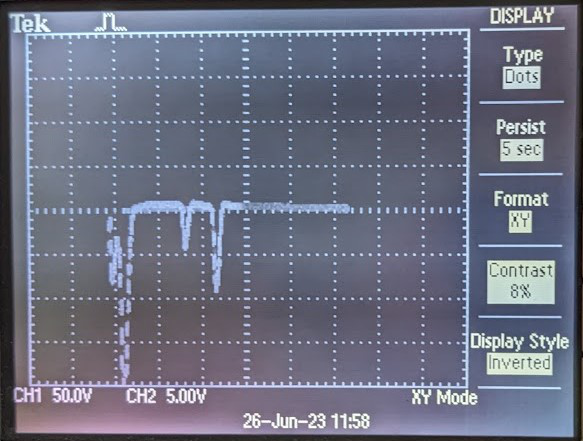
\includegraphics[width = 0.8\linewidth]{pictures/ratio.png}
    \caption{Oszilloskopbild bei $f=\qty{1000}{\kilo\hertz}$.}
    \label{fig:ratio}
\end{figure}
Um das Verhältnis der beiden Isotope zu bestimmen, werden die Tiefen der Absorptionspeaks miteinander verglichen.
Die Tiefe der Peaks gemessen in Pixel auf der Bilddatei betragen für $\ce{^{85}_{}Rb}$ etwa 43px
und für $\ce{^{87}_{}Rb}$ etwa 84px.
Daraus kann das Verhältnis abgeschätzt werden zu
\begin{equation*}
    \frac{^{85}\symup{Rb}}{^{87}\symup{Rb}} \approx 0.51 \, .
\end{equation*}

